\section{Plots}
\begin{itemize}
	\item \textbf{Violin Plot:} These plots represent the density of data as the width at that section. The mean and median of the dataset can be seen clearly. It also shows the symmetry/skewness of the dataset based on the wideness on either side. It shows if the dataset has multiple peaks. It also allows us to compare groups by showing them side by side. It can be used for pharmaceutical trials, ecological studies, financial analysis and quality control.
	      \begin{figure}[H]
		      \centering
		      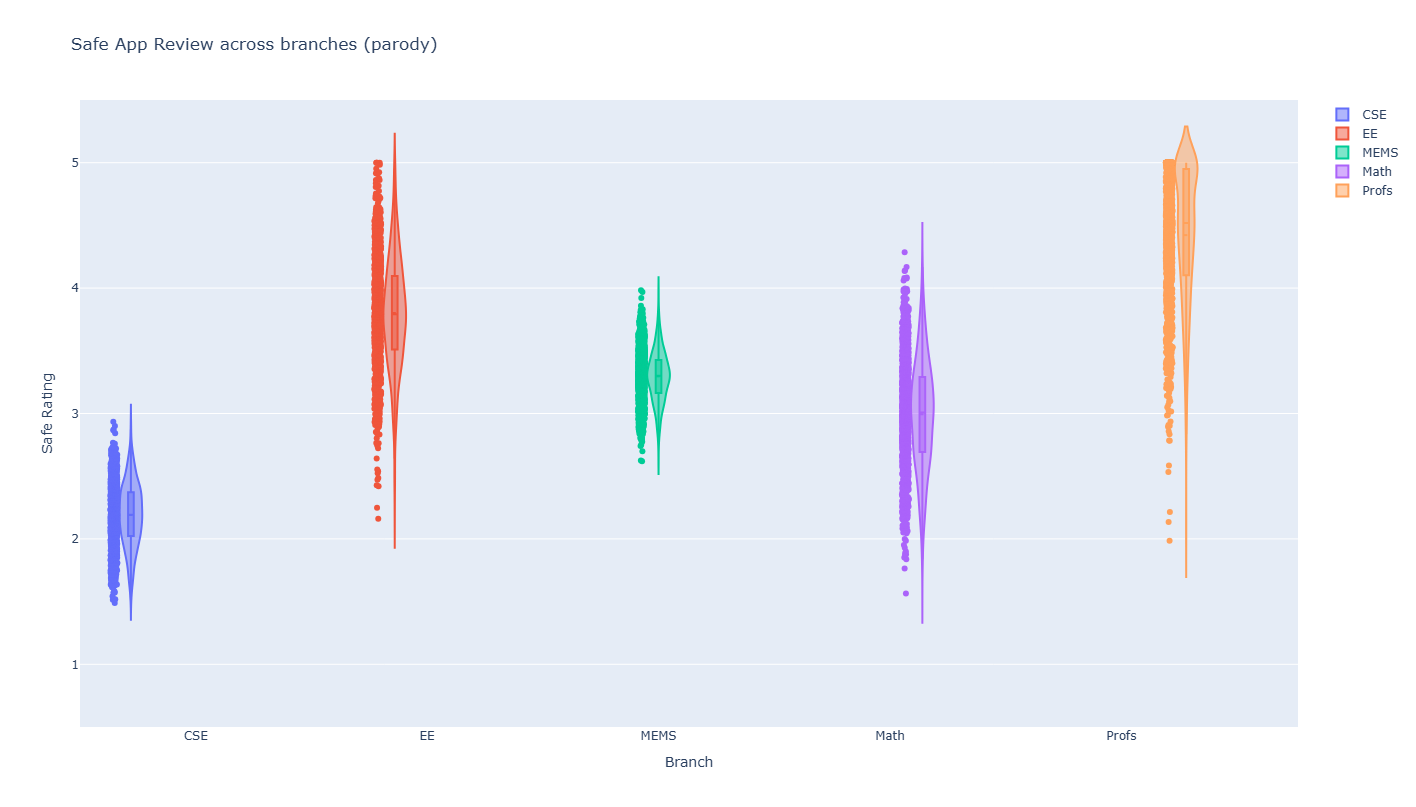
\includegraphics[width=0.85\linewidth]{img/violin.png}
		      \caption{Violin Plot}
	      \end{figure}
	\item \textbf{Pareto Plot:} A Pareto chart is a type of bar chart where each category is represented by a vertical bar. The bars are arranged in descending order of frequency or magnitude from left to right. A cumulative line is often superimposed on the chart to show the total impact of all categories combined. Pareto charts are used to identify the most significant factors in a dataset, typically following the 80/20 rule, where 80\% of the effects come from 20\% of the causes. They are commonly used in quality control, project management, and process improvement to prioritize issues or root causes.
	      \begin{figure}[H]
		      \centering
		      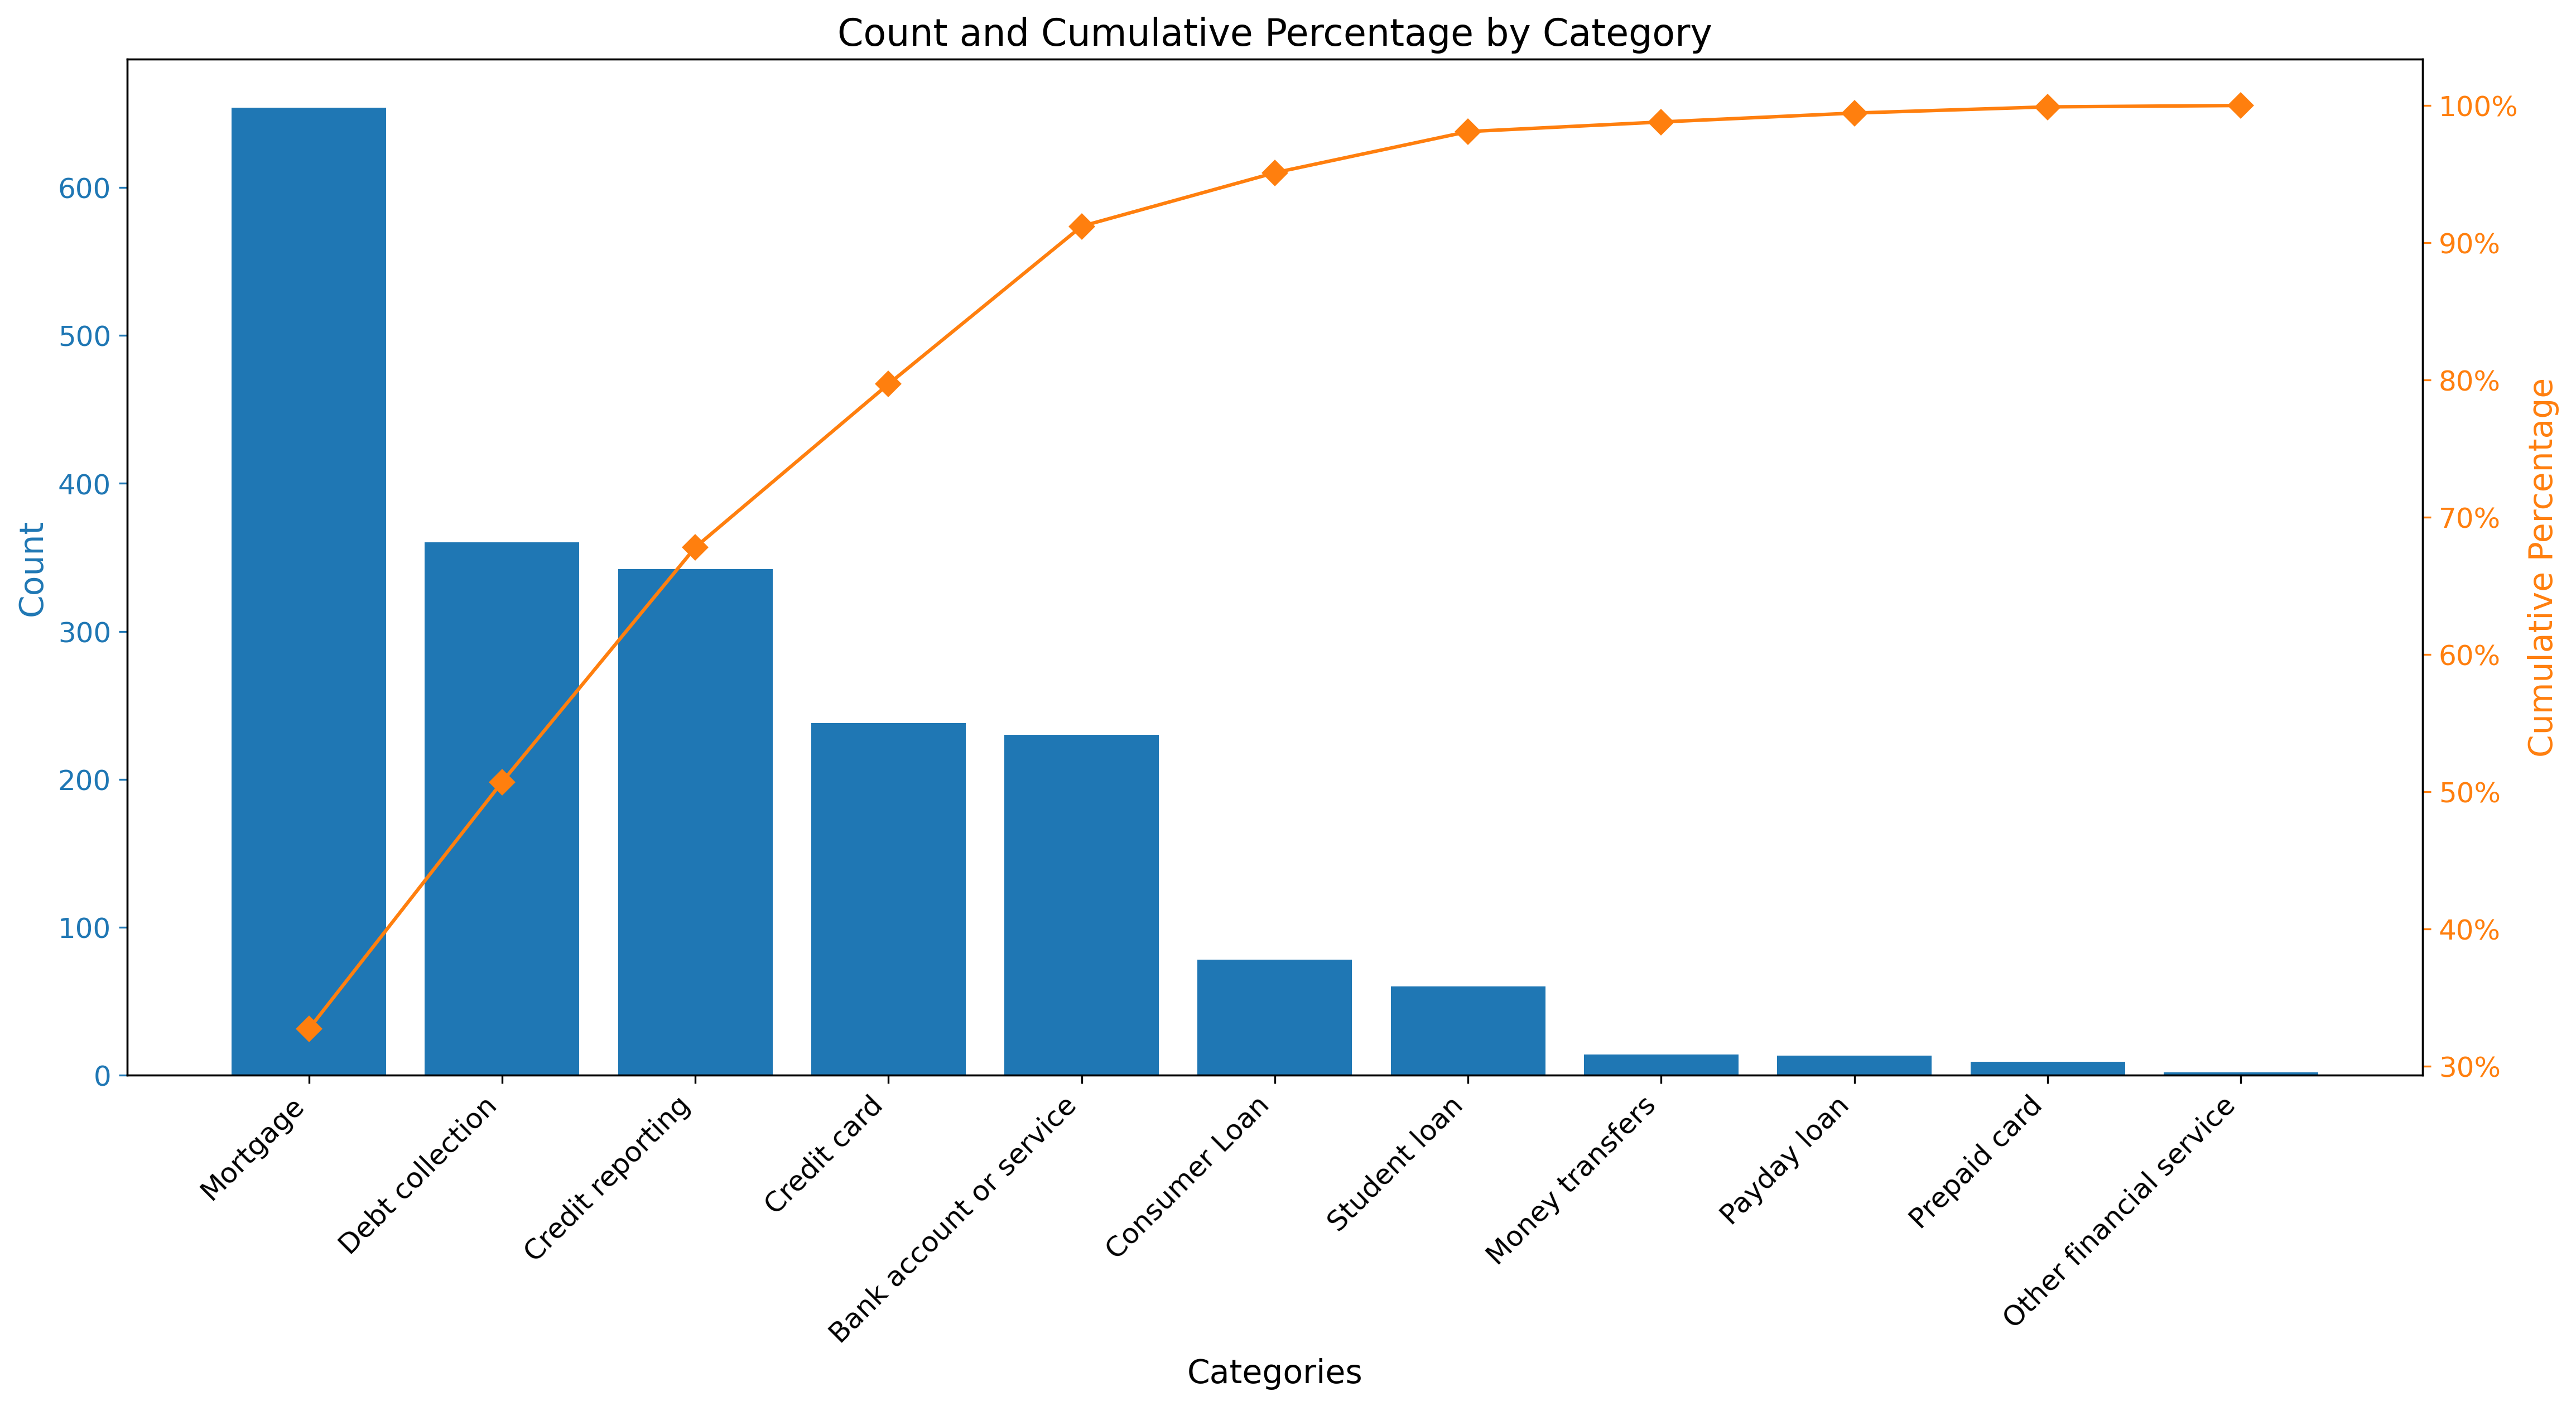
\includegraphics[width=0.85\linewidth]{img/pareto.png}
		      \caption{Pareto Plot, data from \cite{SelenerConsumerComplaints}}
	      \end{figure}
	\item \textbf{Waterfall Plot:} A waterfall plot is a three-dimensional visualization technique commonly used to display changes in signal intensity, frequency, or other continuous variables over time. Each point on the plot represents data at a given time, with the x-axis typically showing time or another independent variable, the y-axis displaying the frequency or another dependent variable, and color or intensity representing the magnitude of the data. Waterfall plots are frequently used in fields such as signal processing, spectroscopy, and audio analysis to monitor how data evolves over time, offering a clear view of trends, patterns, and fluctuations.
	      \begin{figure}[H]
		      \centering
		      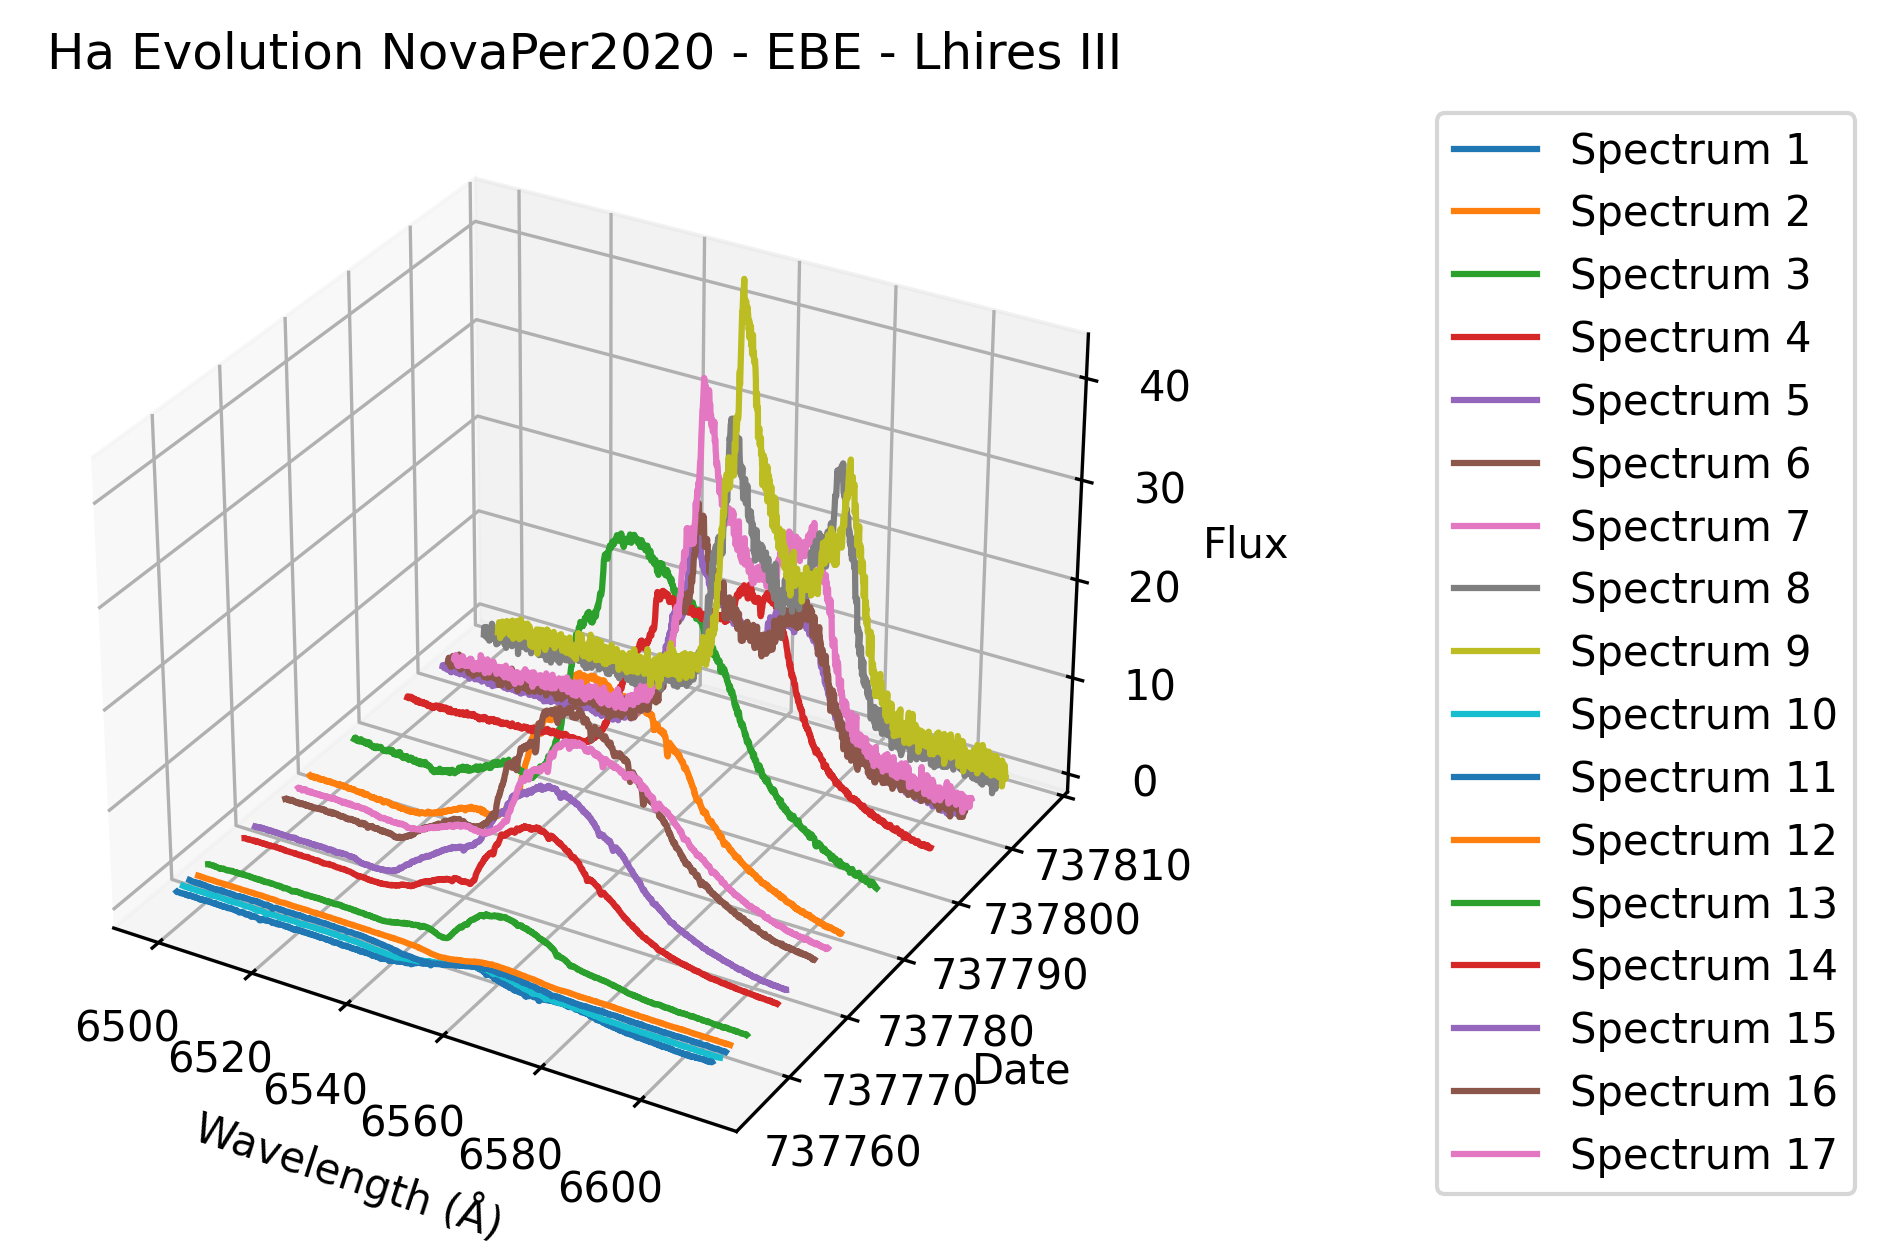
\includegraphics[width=0.8\linewidth]{img/waterfall.png}
		      \caption{Waterfall Plot, data from \cite{Spec3DData}}
	      \end{figure}
	\item \textbf{Coxcomb Plot:} These plots represent data in a circular layout where each category is represented by a wedge. All wedges have the same angular width. Larger areas and longer radii represent larger values and colours are used to represent different time periods. They are used to represent data that changes cyclically like financial performance over the quarters, monthly rainfall or performance of sports players over a season.
	      \begin{figure}[H]
		      \centering
		      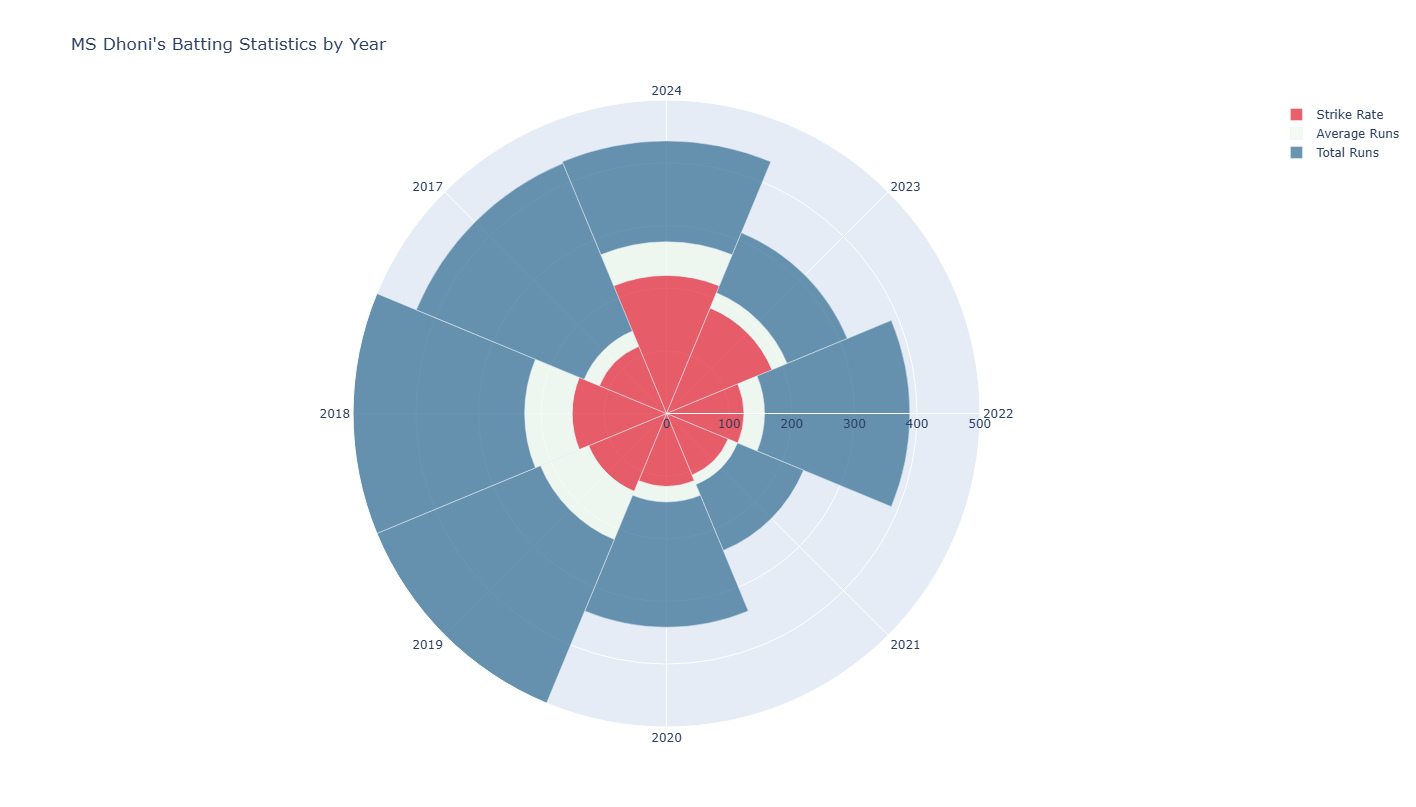
\includegraphics[width=0.85\linewidth]{img/coxcomb.png}
		      \caption{Coxcomb Plot, data from \cite{IPLT20CSKSquad}}
	      \end{figure}


\end{itemize}
